\chapter{Installation et prise en main d'Apache Griffin}
\section*{Introduction}
La qualité est un critère clé pour de nombreuses applications utilisant des données comme l’apprentissage automatique. Cependant, il n’existe pas encore de standard sur la manière dont on pourrait caractériser une "bonne" donnée, ce qui influence grandement la conception des outils. Apache Griffin apparaît comme un dispositif, qui veut redonner confiance aux décideurs qui craignent que des données mal contrôlées puissent avoir un impact négatif sur leurs affaires. Dans ce chapitre, nous allons de prime abord pr\'esenter l'outil, une description de son installation ainsi que les processus ayant permis sa prise en main et enfin nous terminerons par une ouverture sur ses limites et perspectives.
\section{Pr\'esentation de Apache Griffin}


\subsection{Aperçu de l'outil}
Apache Griffin, est une solution open source de qualit\'e des donn\'ees pour le \textit{big data}. Il est d\'ecrit par ses concepteurs comme \'etant une plateforme offrant des services de qualit\'e des donn\'ees. De ce fait, il fournit un cadre complet d'analyse, permettant de r\'ealiser diverses t\^aches telles que la d\'efinition d'un mod\`ele de qualit\'e des donn\'ees, le calcul de diverses m\'etriques, l'automatisation de la validation des donn\'ees ainsi qu'une visualisation unifiée des m\'etriques. Gr\^ace aux infrastructures composant son \'ecosyst\`eme, Apache Griffin (Griffin) permet de g\'erer des donn\'ees venant aussi bien en temps r\'eel (\textit{streaming}) que par lot (\textit{batch}), tout en relevant les d\'efis en mati\`ere de qualit\'e dans les applications \textit{big data}. Face \`a l'absence de consensus sur la qualit\'e, Apache Griffin propose un standard sans pour autant \^etre restrictif.
\\

Conçu dans les locaux d'eBay en Mars 2016, puis confi\'e \`a la fondation Apache le 7 D\'ecembre de la m\^eme ann\'ee, Apache Griffin venait combler un certain nombre de besoins notamment \cite{ApacheGriffinIntro} : 
\begin{itemize}[parsep=0cm,itemsep=0cm]
\item le suivi de la qualit\'e  depuis de multiples sources de donn\'ees jusqu'aux applications cibles, tout en tenant compte de leurs historiques;

\item l'\'evaluation de la qualit\'e des donn\'ees en \textit{streaming} et en \textit{batch} tout en offrant la possibilit\'e de suivre l'évolution des diff\'erentes m\'etriques;

\item la mise en place d'une plateforme exposant une \acrshort{api}, permettant aux développeurs d'impl\'ementer leur propre interface utilisateur.
\end{itemize}

\subsection{Fonctionnalit\'es  d'Apache Griffin}

Afin de satisfaire ces diff\'erents besoins, Apache Griffin propose de nombreuses fonctionnalit\'es. Telles que pr\'esent\'ees dans la documentation, nous avons: 

\begin{itemize}[parsep=0cm,itemsep=0cm]

\item \textbf{la d\'efinition de mesures} : l'exactitude, l'exhaustivité ou la compl\'etude, l'actualité, l'unicité, la validité, la cohérence; il s'agit des diff\'erentes dimensions de la qualit\'e des donn\'ees qui peuvent \^etre \'evalu\'ees. L’utilisateur peut créer, modifier, supprimer et planifier des jobs pour les données venant par batch ;

\item \textbf{la surveillance des anomalies} : l'\'etablissement d'attentes sp\'ecifiques pour détecter les données anormales, tout en offrant la possibilit\'e de les téléchargés  ;

\item \textbf{les alertes en cas de d\'etection d'anomalies} : signaler les problèmes de qualité des données par e-mail ou sur la plateforme;

\item \textbf{la surveillance visuelle} : gr\^ace \`a son interface web, on peut appr\'ecier l'\'etat de la qualité des données au fil du temps;

\item \textbf{le temps réel} : l'inspection de la qualité des données peut être effectuée en temps réel;

\item \textbf{l'\'elasticit\'e et l'agilit\'e} : gr\^ace \`a ses facult\'es, Griffin peut être utilisé pour l'analyse des données provenant de plusieurs entrepôts de données. De plus, il fonctionne dans un environnement (Spark et Hadoop) pouvant g\'erer de grands volumes de donn\'ees (1,2 Petaoctet soit 1000 T\'eraoctet, cas d'eBay);

\item \textbf{la simplicit\'e} : Griffin fournit une interface utilisateur simple et facile à utiliser qui peut gérer les données et les règles de qualité; en même temps, les utilisateurs peuvent visualiser les résultats de qualité des données et personnaliser le contenu de l'affichage par le biais du panneau de contrôle.

\end{itemize}

\begin{figure}[H]
  \caption{Fonctionnalit\'es de Apache Griffin}  \label{fig:xray}
  \begin{center}
    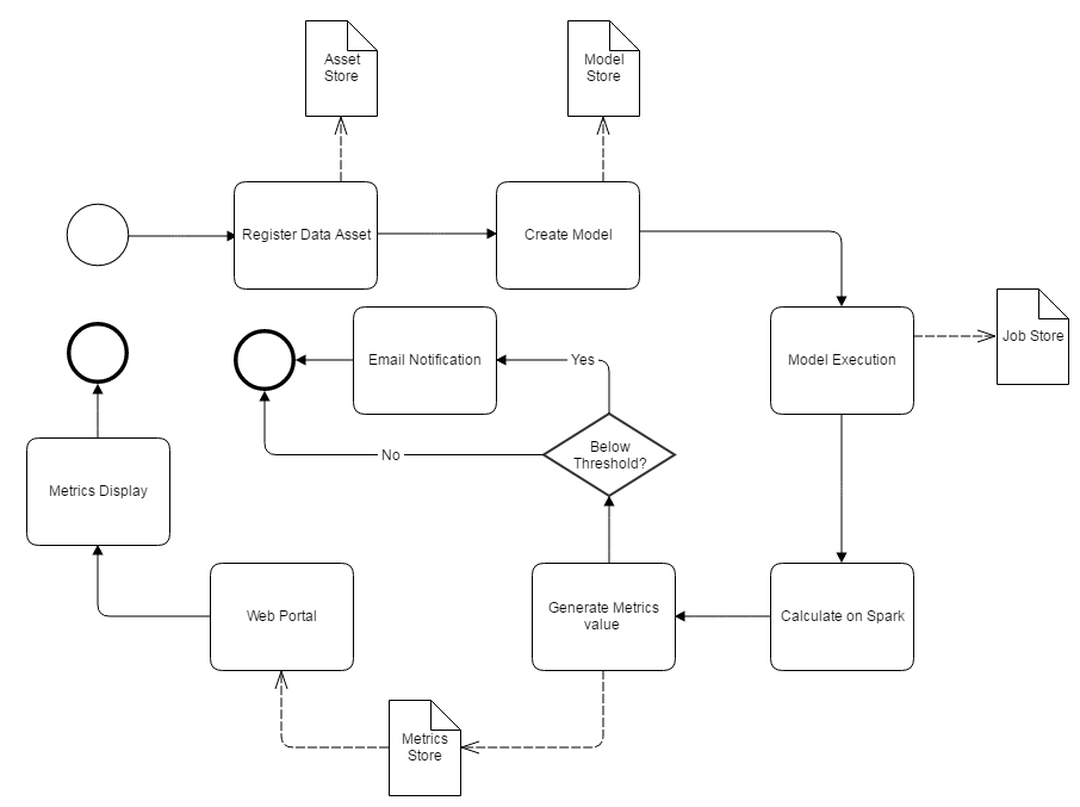
\includegraphics[scale=0.45]{Static/Capture.png} 
  \end{center}
\end{figure}

\subsection{Dimensions de la qualit\'e de donn\'ees}
 Dans cette sous-section, nous mettrons l'accent sur les langages de qualit\'e des donn\'ees de Griffin et sur les dimensions impl\'ement\'ees. En effet, les règles de qualit\'e des donn\'ees de Griffin sont \'edit\'ees soit \`a l'aide de  \emph{griffin-dsl} ou du \emph{spark-sql}. Tous deux ont pour syntaxe de base le \acrshort{sql}. Le \emph{griffin-dsl} est une surcouche du \emph{spark-sql}, mais moins verbeuse que ce dernier. Il suffit de pr\'eciser quelques mots cl\'es en fonction de la dimension choisie pour \'etablir la r\`egle voulue. Elle est ensuite traduite en \emph{spark-sql} puis ex\'ecut\'ee sur Apache Spark. Le \emph{spark-sql} est issu du module Spark \acrshort{sql} d'Apache Spark permettant de travailler avec des données structurées. Il permet de faire des requ\^etes sur Spark mais en utilisant le langage \acrshort{sql}, et cela peu importe la structure des donn\'ees. \\

Griffin offre \'egalement un certain formalisme en termes de qualit\'e des donn\'ees, dans la mesure o\`u il impl\'emente déjà en son sein plusieurs dimensions. Elles sont d\'efinies pour l'utilisation de \emph{griffin-dsl}. Au nombre de ces dimensions nous avons : 

\begin{description}[parsep=0cm,itemsep=0cm]
\item[Accuracy] : on cherche \`a obtenir le nombre de correspondances entre une donn\'ee source et une donn\'ee cible, conform\'ement \`a la dimension Exactitude. La d\'efinition de la règle décrit la relation de mappage entre les deux sources de données. Par exemple on a : "source.id = target.id and source.name = target.name";
\item[Profiling] : cette dimension permet de faire un profilage des donn\'ees. L'\'ecriture de la r\`egle peut se faire au moyen du langage \acrshort{sql} (\emph{spark-sql}) ou en \'ecriture simplifi\'ee (\emph{griffin-dsl}) comme: "source.id.count(), source.age.max() group by source.country";
\item[Distinctness] : il s'agit d'identifier les données qui sont en double (dimension Unicité). Pour ce faire, il suffit de pr\'eciser la ou les colonne(s) cibl\'ees s\'epar\'ees d'une virgule: "name, age";
\item[Completeness] : on vérifie ici si les valeurs d'une ou plusieurs colonnes sont nulles (dimension Exhaustivité). La r\`egle s'\'ecrit juste en pr\'ecisant la ou les colonnes dont on veut \'evaluer la compl\'etude;
\item[Timeliness] :  cette impl\'ementation mesure la latence de chaque élément et donne des statistiques de latence. Elle est disponible uniquement pour les donn\'ees en \textit{streaming}.
\end{description}
L'usage de \emph{spark-sql} peut \^etre vu comme un mode expert ou avanc\'e. Toutefois, la version 0.6.0 d'Apache Griffin n'offre que l'impl\'ementation de l'Accuracy, du Profiling et de la Completeness pour le \emph{griffin-dsl}. Pour l'impl\'ementation de nos r\`egles de qualit\'e nous avons fait une combinaison de \emph{spark-sql} et de \emph{griffin-dsl}.

\subsection{Architecture d'Apache Griffin}
\subsubsection{\textbf{Modules}}
L'outil est constitu\'e de trois (3) principaux modules : UI, Service, Measure. Le module UI pour \textit{User Interface}, est d\'evelopp\'e avec le \textit{framework} javascript Angular JS. Il s'agit du module qui g\`ere l'interface graphique de Apache Griffin. Il permet la visualisation des m\'etriques, leurs d\'efinitions et ordonnancement. Tout ceci est possible gr\^ace aux communications avec l'\acrshort{api} Service via le protocole \acrfull{http}. 
 %\begin{figure}[h]
 %   \begin{center}
 %     
\includegraphics[scale=0.65]{Static/create measure.png} 
%	\end{center}
%	\caption{Cr\'eation d'une mesure sur l'UI de Apache Griffin}  \label{fig:xray}
 %\end{figure}
 
\begin{figure}[H]
    \caption{UI de Apache Griffin} \label{fig:xray}
    \begin{center}
      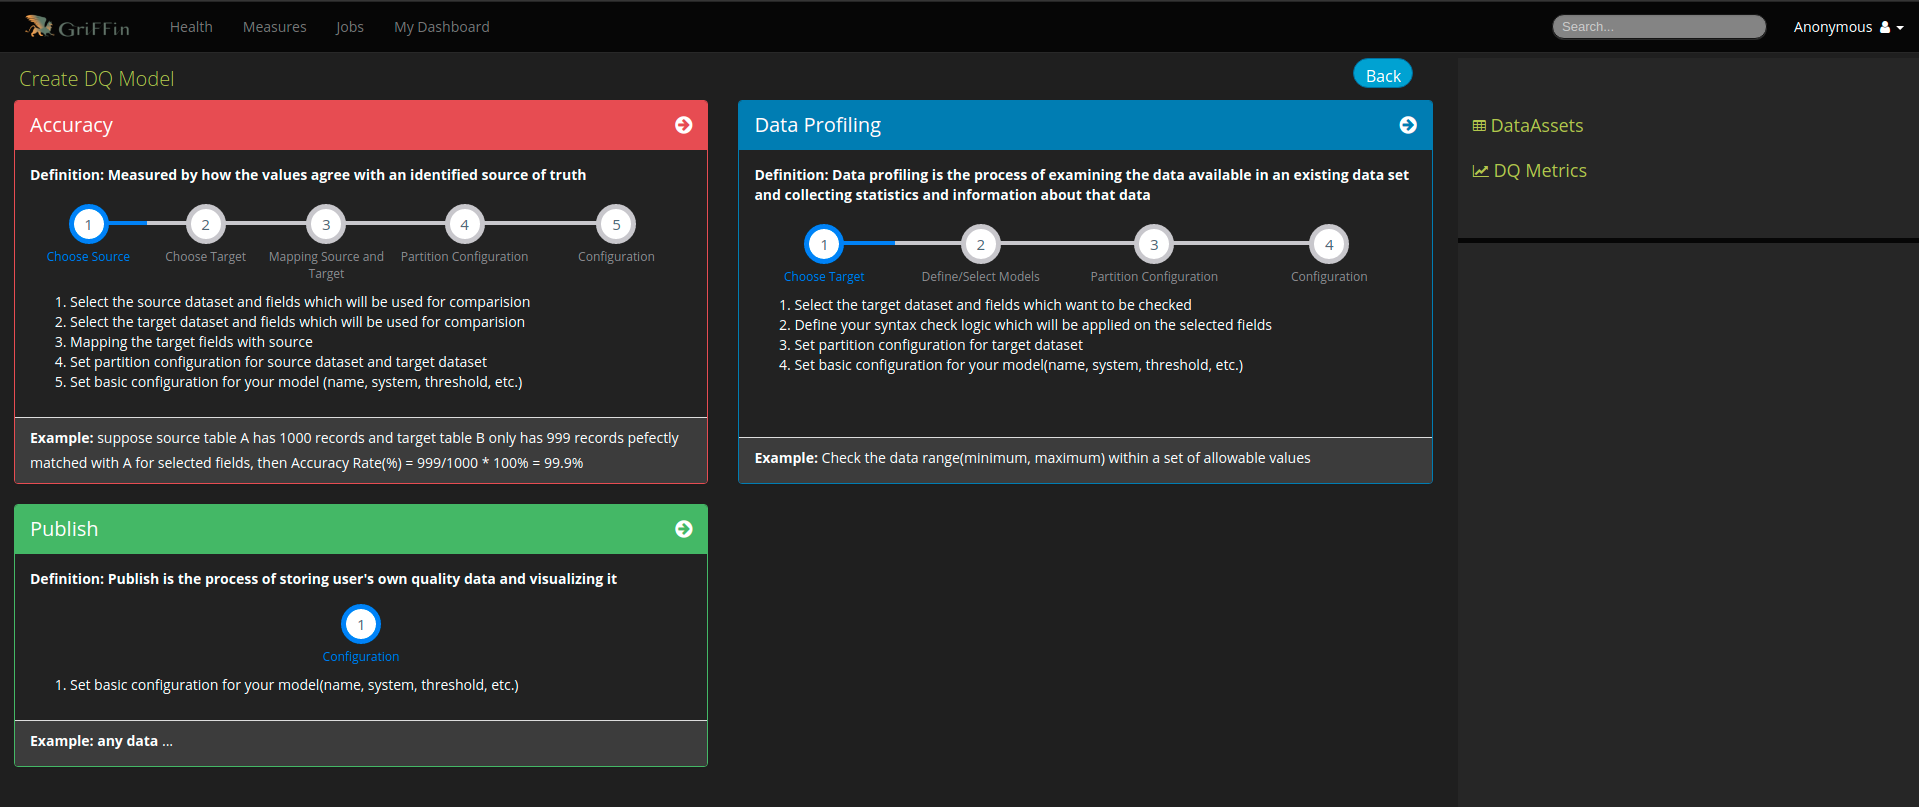
\includegraphics[scale=0.25]{Main/Static/UI_griffin.png} 
     \end{center}
\end{figure}
Le module Service, repr\'esente donc le web service de Apache Griffin. Développé en Java avec le \textit{framework} Spring Boot, il expose une \acrshort{api} \acrshort{rest}ful tr\`es riche. Elle offre bien plus de possibilit\'es qu'une utilisation via l'interface graphique, mais dans ce cas n\'ecessite de faire recours \`a un client tel que Postman pour les tests. Le calcul des diff\'erentes m\'etriques est fait par le module Measure, qui quant \`a lui est \'ecrit en Scala. 
\\
\begin{figure}[H]
    \caption{Interroger Apache Griffin avec Postman} \label{fig:xray}
    \begin{center}
      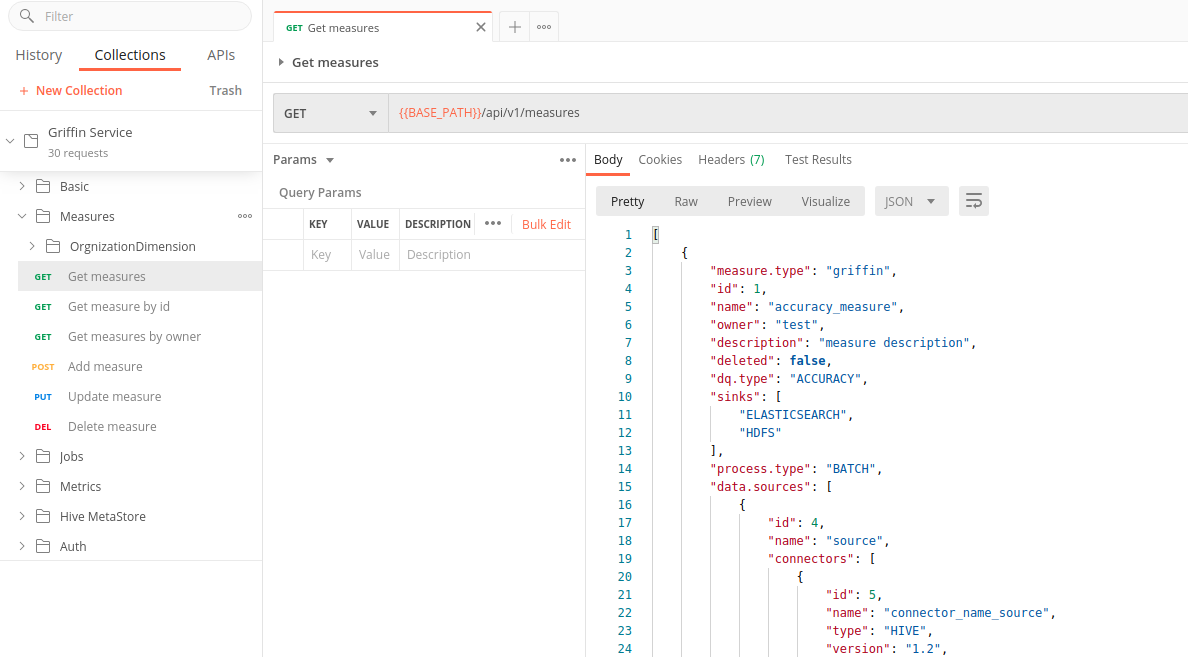
\includegraphics[scale=0.35]{Main/Static/Postman_Griffin.png} 
     \end{center}

\end{figure}
 
%\newpage
\subsubsection{\textbf{Couches de fonctionnement de Apache Griffin}}

Une vue m\'eso de l'architecture de Apache Griffin met en \'evidence trois (3) principales couches: Analyze, Measure et Define chacune jouant un r\^ole fondamental dans le fonctionnement de Griffin. D'abord, nous avons la couche Define, qui est responsable de la d\'efinition des dimensions de qualit\'e. Ensuite, vient la couche Measure qui permet le calcul des diff\'erentes m\'etriques. Les r\'esultats sont stock\'es dans le r\'ef\'erentiel de la derni\`ere couche : Analyze. Elle s'occupe de la sauvegarde et de l'affichage des r\'esultats. 

\begin{figure}[!h]
    \caption{S\'equences de fonctionnement de Apache Griffin}  \label{fig:xray}
    \begin{center}
      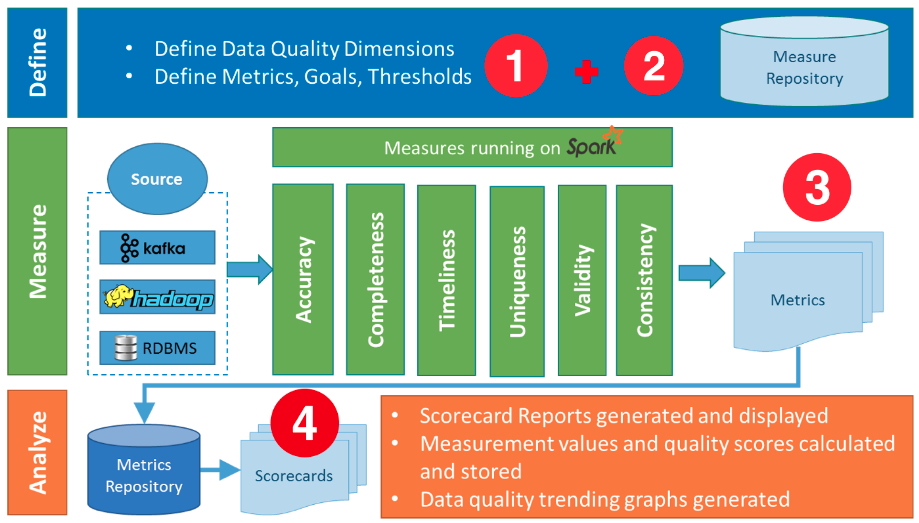
\includegraphics[scale=0.5]{Main/Static/Sequences_de_fonctionnement_Griffin.png} 
    \end{center}
\end{figure}
Suivant cette architecture, on a un flux de travail se pr\'esentant comme suit :

\begin{enumerate}[parsep=0cm,itemsep=0cm]
\item Enregistrement de la source ou des sources de données ;
\item Configuration des r\`egles de qualit\'e, qui peuvent être définies à partir des dimensions de qualité de données ;
\item Planification  de la tâche à soumettre p\'eriodiquement au \textit{cluster} Spark et stockages des m\'etriques;
\item Visualisation des indicateurs sur l'interface et analyser le rendu : la carte thermique et le tableau de bord peuvent \^etre utilis\'es \`a cet effet.

\end{enumerate}
\vspace{0.2cm} 

\subsubsection{\textbf{Infrastructures de l'écosystème d'Apache Griffin}}
Au niveau micro, Apache Griffin est un outil qui d\'epend et utilise plusieurs autres infrastructures \textit{big data} pour l'ex\'ecution des t\^aches. Nul besoin de pr\'eciser qu'on ne saurait parler d'infrastructures \textit{big data} sans citer Apache Hadoop et Apache Spark en premier lieu. Ainsi on y trouve les applications suivantes :

\begin{itemize}[parsep=0cm,itemsep=0cm]
\item \textbf{Apache Hadoop} (version 2.6.0 ou plus) : c'est un \textit{framework} de stockage et de traitement distribu\'e de grands ensembles de donn\'ees sur des \textit{clusters} d'ordinateur. Il sert de source de donn\'ees et au stockage des m\'etriques pour les traitements \textit{batch}. Toute l'architecture repose sur Hadoop;

\item \textbf{Apache Spark }(version 2.2.1 ou plus ): c'est un moteur de calcul distribu\'e et de traitement rapide des donn\'ees, d\'edi\'e au \textit{big data}. Le calcul des m\'etriques est effectu\'e sur Spark pour un gain maximal de performance ;

\item \textbf{Apache Hive} (version 2.x ): il s'agit d'un entrep\^ot de donn\'ees qui sert de \textit{metastore} et \'egalement de source de donn\'ees pour Griffin;

\item \textbf{PostgreSQL} (version 10.4 ou plus) ou \textbf{MySQL} (version 8.0.11 ou plus) :  ce sont des Syst\`emes de Gestion de Bases de Donn\'ees Relationnelles qui servent ici au stockage des diff\'erentes configurations en termes de dimensions de qualit\'e  et ainsi que les d\'etails concernant l'ex\'ecution (model store, asset store, job store) ;

\item \textbf{Livy} : permet de soumettre de façon programmatique des jobs spark  depuis des applications web/mobiles. Il s'agit d'une \acrshort{api} \acrshort{rest}ful ;

\item \textbf{Elasticsearch} (version 5.0 ou plus ): quant \`a lui permet \'egalement de stocker les r\'esultats (m\'etriques) issus de l'analyse de la qualit\'e des donn\'ees;

\item \textbf{Kafka} : Kafka est utilisé principalement pour la mise en place de flux de donn\'ees en temps réel.

\end{itemize}
%\vspace{0.15cm}
Griffin int\`egre \'egalement les d\'ependances suivantes : 

\begin{itemize}[parsep=0cm,itemsep=0cm]
\item \textbf{JDK} pour \acrlong{jdk};
\item \textbf{Scala};
\item \textbf{Maven} qui est un outil de  gestion de projet, utilisé pour empaqueter le projet Apache Griffin en fichier \textit{.jar};
\end{itemize}
\section{Installing and connecting Griffin to PostgreSQL}
\subsubsection{Tool installation}
To install Apache Griffin and make the configurations, we used the following architecture:
\begin{figure}[H]
    \caption{Architecture implemented to test Apache Griffin}  \label{fig:xray}
    \begin{center}
      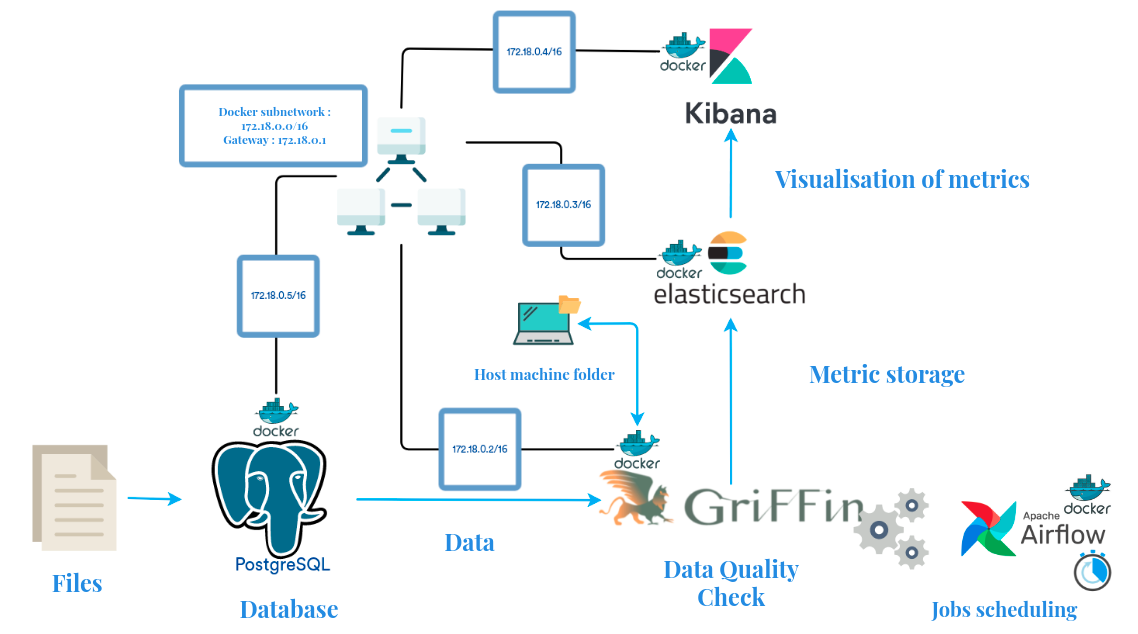
\includegraphics[scale=0.40]{Main/Static/Arch_eng.png} 
    \end{center}
\end{figure}
The installation is done via docker and takes place in two main steps, according to the documentation \cite{ApacheGriffinDocDocker}. First, a preparation of the working environment is required. This step is carried out in three (3) essential points:
\begin{enumerate}[parsep=0cm,itemsep=0cm]
    \item the installation of docker and docker compose;
    \item increasing the virtual memory limits for the use of Elasticsearch;
    \item retrieving the docker images needed for the installation. 
\end{enumerate}
After preparing the environment, the next step is the creation of the different docker containers.

\subsubsection{Connection to PostgreSQL}
Assessing the quality of data obviously requires data. For this purpose, Griffin allows you to configure access to different data sources. In particular, in batch mode, Griffin can audit the quality of data located in Hive tables, AVRO files, flat files (Parquet, \acrfull{csv}, \acrfull{tsv}, \acrfull{orc}) and data from sources with \acrshort{jdbc} (\acrlong{jdbc}) drivers such as Oracle, MySQL, PostgreSQL, etc. However, the connection to a PostgreSQL database was not natively supported.  To remedy this, we have modified the source code of the application. This modification involves adding the PostgreSQL database connection driver to the project dependencies. Then at the level of the test files, it was necessary to adapt the code, so that at the phase of build of the project, the driver once downloaded is suitably added to the Classpath. 

\section{Evaluation of the quality of the Digital Factory's data}
The second phase of the project aims to evaluate the quality of some tables with Griffin and to propose corrective measures where possible. For this purpose, two data extractions were provided. These are the 'Detail\_Victimes' and 'Inventaire\_Sinistre' tables. The 'Detail\_Victimes' table contains the information of all deceased or injured victims of an insurance claim as well as the differents assessments history. The 'Inventaire\_Sinistre' table contains the entire claim inventory, including settlements, reserves, and recoveries. The results of the evaluation are presented along each dimension.

\subsubsection{Uniqueness dimension}
For this dimension, we also highlighted for each targeted column three (3) metrics: the total number of observations in the column, the number of distinct observations and the number of distinct observations appearing more than once. The results of this assessment revealed that there were repetitions in the different columns. However, this did not constitute anomalies. This is due to the fact that the data is derived from the join between several tables.

\subsubsection{Validity dimension}
In this dimension we evaluated three (3) main rules. The objective was to identify the range of variation of the quantitative columns, to define the modalities of the different qualitative columns and to highlight the values presenting problems of encoding of accentuated characters. As a result of the evaluation,  we have highlighted encoding problems in the \textit{'Beneficiaire'} column of the 'Detail\_Victimes' table. The encoding problems as we detected them are characterised by the appearance of '?' in place of accented characters. Thus 'p\`ere' is spelled out as 'p?re' for example.

\subsubsection{Completeness dimension}
We use three (3) metrics to assess this dimension: the total number of rows, the number of incomplete observations and the number of non-zero observations. We have eighty (80) columns with missing values for 'Detail\_Victimes'  i.e. about 86\% of the table's columns, and 39 columns for 'Inventaire\_Sinistre', i.e. about 43\% of the columns.

\begin{figure}[H]
    \caption{Completeness 'Detail\_Victimes'}  \label{fig:xray}
    \begin{center}
      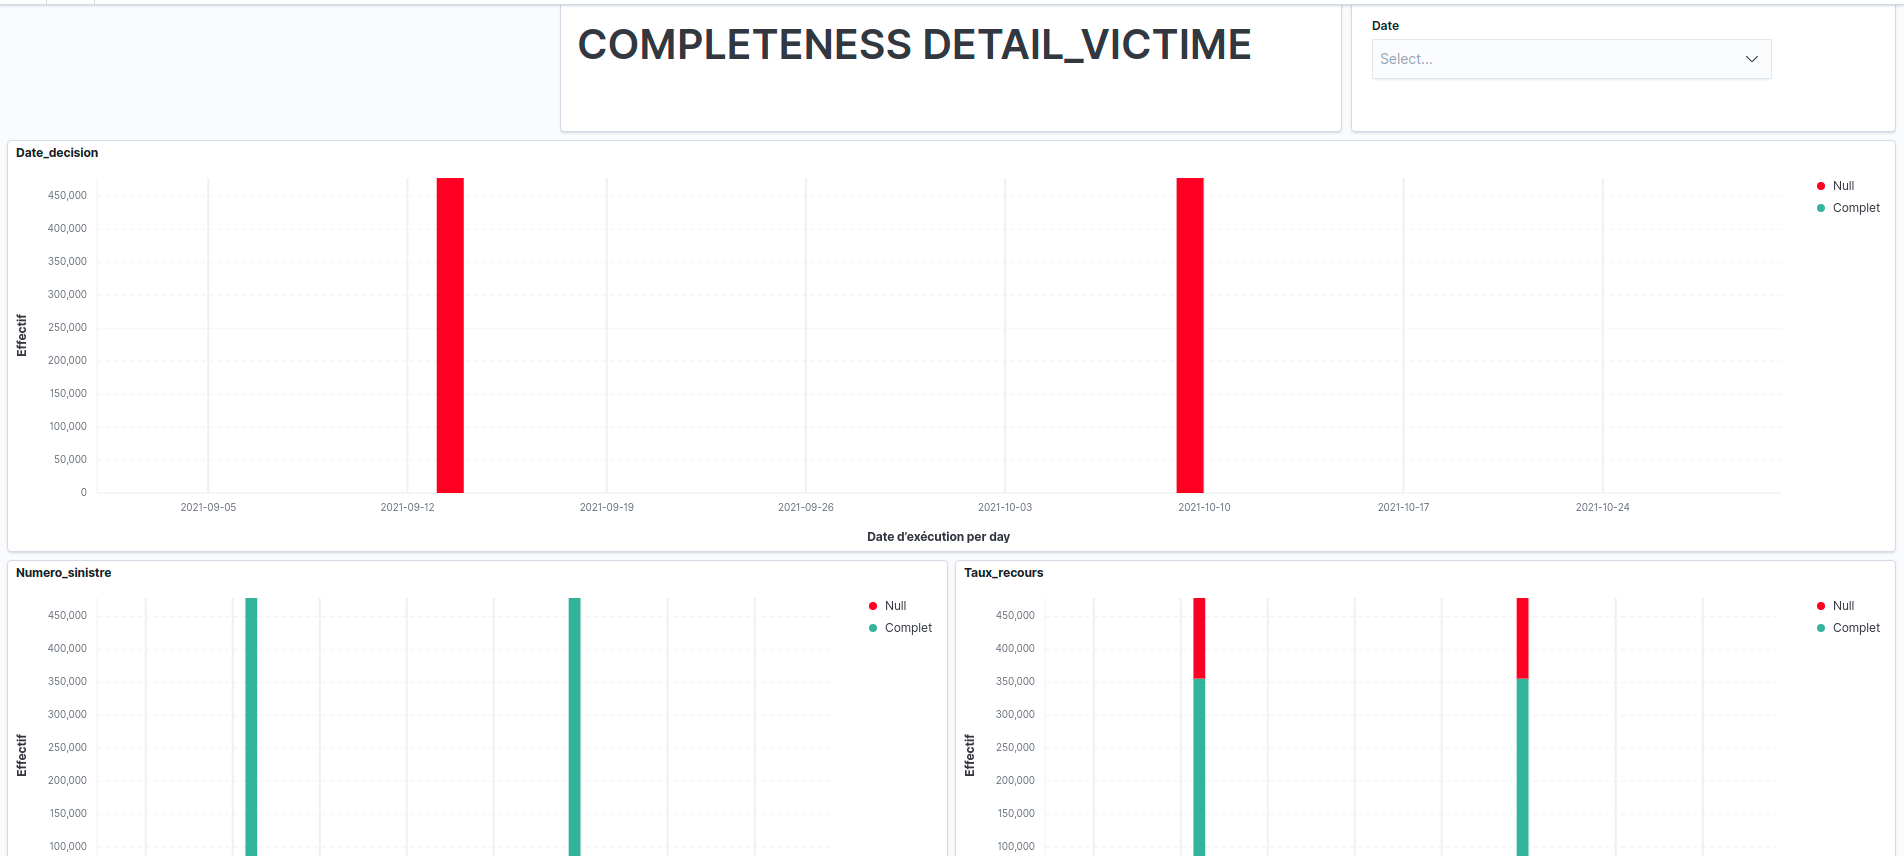
\includegraphics[scale=0.27]{Main/Static/Completeness_Detail_Victime.png} 
    \end{center}
\end{figure}



\subsubsection{Consistency Dimension}
\textbf{'Inventaire\_Sinistre' table}\\
The rules established at the level of this dimension, allow to attest the consistency of the data with the business rules. It is expected that the formulas for the calculation of the charge, the total settlement and the total provision are respected. We also checked the consistency of the dates. Logically, the date of occurrence of the claim, the date of opening of the file and the date of birth of the driver should be earlier than the date of declaration of the claim, the date of closure and the date of licence respectively. In addition to these rules, we have assessed the consistency of the nature of the claim, whether it is 'Bodily' or 'Material'. Indeed, a claim that results in injury and/or loss of life cannot be classified as 'Material'. On the other hand, some claims may be classified as 'Bodily' if they cost more than 100,000 Moroccan dirham even though there are no injuries or deaths. These different rules make it possible to assess the consistency of the nature of the claim. We discovered : 
\begin{itemize}[parsep=0cm,itemsep=0cm] 
    \item 1 claim of a 'Material' nature but with 5 injured victims and 1 deceased;
    \item 237,657 claims with a cost of less than 100,000 Moroccan dirham, with no victims recorded but of a 'Bodily' nature;
    \item 190,622 claims where the number of victims is unequal to the count in the 'Detail\_Victimes' table;
    \item 102 observations for which the claim is declared before it occurs;
    \item 3,972 observations for which the date of obtaining a driving licence is earlier than the date of birth;
    \item 76,000 observations with file opening dates chronologically later than the file closing date.
\end{itemize}
\textbf{'Detail\_Victimes' table}\\
We verify whether the amounts of medical and pharmaceutical expenses and those of permanent partial disability are correctly entered, in accordance with the amount indicator variables. A check has also been made on the consistency of the date of occurrence and declaration. The execution of the rules revealed the following results: 19,082 observations are affected by an inconsistency between the dates of occurrence and declaration. Moreover, when the indicator variable takes the value 'N', meaning that there should be no expenses (medical and pharmaceutical or permanent partial disability), there is sometimes an amount present.

\section{Correction and quality improvement}
The review of the state of data quality identified columns with various anomalies. However, not all of these anomalies constitute errors. Once the selection had been made, we undertook to apply corrections to the columns with consistency problems, as well as a correction of the encoding problems. The various corrections were applied using PySpark (version 2.4.7). This is a Python interface for Apache Spark. 

\subsubsection{Reliability of the number of victims and the nature of the disaster}
In order to correct the differences in the number of injured and deceased victims in the 'Inventaire\_Sinistre' table, the number of injured and deceased victims was counted for each loss in the 'Detail\_Victimes' table. This new data, together with the information contained in the 'Inventaire\_Sinistre' table, produced a new column giving the number of injured and dead for each claim with a corresponding value in the 'Detail\_Victimes' table. With these new values, we proceeded to adjust the nature of the incident. If the number of injured or dead is greater than zero (0), then the claim type is 'Bodily'. Otherwise, if the charge is less than or equal to 100,000 Moroccan dirham and the claim was previously classified as 'Bodily', it is reclassified as 'Material'. Indeed, there is no reason to consider it as a 'Bodily' claim. On the other hand, if none of the above conditions are met and the charge is strictly greater than 100,000 Moroccan dirham or a claim of a 'Material' nature, then the value of the initial variable \textit{'Nature\_Sinistre'} is retained. This adjustment algorithm leads to the creation of a new variable \textit{'Nature\_Sinistre\_New'}.

\subsubsection{Algorithm for correcting encoding problems}
The targets of our correction are the words of the dictionary (not the proper names). The algorithm algorithm used uses Levenshtein's distance to identify the most likely spelling corrections for a word : these are the candidate words. Levenshtein's distance is a measure of similarity between two strings. It is equal to the number of elementary operations to do to transform a string M into a string P. These are :
\begin{itemize}[parsep=0cm,itemsep=0cm]
    \item substitution of a character ;
    \item insertion or addition of a character ;
    \item deleting or erasing a character.
\end{itemize}

Once the list of candidate words has been obtained, the algorithm then compares all the candidates with a dictionary of words. The particularity of this dictionary is that it associates each word with a frequency of occurrence. The key is the word and the value is the frequency of the word. The candidate with the highest frequency of occurrence is more likely to be the correct result. In case of co-occurrence an alphabetical ranking is performed. This algorithm is implemented in Python by the SpellChecker library. 

\subsubsection{Reliability of indicator variables}
Any amount strictly greater than zero (0) must be materialized by the modality 'Y' in the indicator variable. The correction of these inconsistencies is therefore done using the following algorithm: if the amount is greater than zero (0), a new indicator variable is assigned the value 'Y'. Otherwise, the value 'N' is returned to indicate that there is no charge. The correction results in the creation of a new column so that the existing data is not altered. The algorithm implemented allowed the correction of inconsistencies and the imputation of missing values of indicator variables.
\section{Limites et perspectives d'Apache Griffin}

La documentation d'Apache Griffin fournit une feuille de route sur les prochaines fonctionnalit\'es \`a d\'evelopper ainsi que celles disponibles. N\'eanmoins, certaines fonctionnalit\'es actuellement disponibles, pr\'esentent les limites suivantes: 
\begin{description}[parsep=0cm,itemsep=0cm]
\item[la gestion des mesures] : En effectuant des op\'erations sur l'interface utilisateur, on ne peut que cr\'eer, supprimer et mettre \`a jour que trois types de mesures. Les appels par l'\acrshort{api}, offrent \`a l'utilisateur un panel plus vari\'e de mesures (accuracy, profiling, timeliness, uniqueness ou distinctness, completeness, publish metrics). Toutefois l'absence d'impl\'ementation de connecteur de type \acrshort{jdbc} au niveau du web service limites assez la vari\'et\'e des sources;

\item[la gestion de l'ex\'ecution des mesures (jobs)]: L'utilisateur ne peut créer, modifier, supprimer et  planifier des jobs pour les donn\'ees venant par \textit{batch}, uniquement que pour les mesures \'elabor\'ees pour les connexions de type HIVE, AVRO, CUSTOM, via Postman. 
\end{description}
De plus, la mesure de type Uniqueness pr\'esente quelques dysfonctionnements et la Publish Metrics n'est pas document\'ee, faute de quoi nous n'avons pas pu la tester. Pour cette derni\`ere nous soupçonnons une obsolescence de la fonctionnalit\'e. Car m\^eme dans le code source elle s'est av\'er\'ee absente. Notons \'egalement que la documentation sur github bien que d\'etaill\'ee, n'est pas tenue \`a jour. 
\\

\`A court-terme, Apache Griffin envisage de supporter plus de sources de donn\'ees. Notamment un enrichissement de la connexion aux bases de donn\'ees relationnelles, ainsi qu'une connexion \`a Elasticsearch. De plus, Griffin pr\'evoit prendre en charge de mani\`ere native d'autres dimensions de qualit\'e de donn\'ees comme la coh\'erence et la validit\'e. Pour l'instant, il est laiss\'e \`a la charge de l'utilisateur la d\'efinition des attentes vis-\`a-vis de ces dimensions. Une nouvelle fonctionnalit\'e est \'egalement cibl\'ee:  il s'agit de la d\'etection d'anomalie en analysant les m\'etriques calcul\'ees par Elasticsearch. Notons \'egalement que dans le cadre de cette \'etude, nous avons utilis\'e la version 0.6.0 d'Apache Griffin, mais durant cette exploration, de nouvelles fonctionnalités et des am\'eliorations de celles existantes ont \'et\'e publi\'ees sur github. Il s'agit de la réécriture et de la red\'efinition des diff\'erentes dimensions. Ainsi la nouvelle version s'appuiera probablement sur les dimensions suivantes :  l'Accuracy, la Completeness, la Duplication et le Profiling. En plus, de ces quatre dimensions Griffin intègre une nouvelle: la conformit\'e du sch\'ema. Cette mesure \'evalue si oui ou non les donn\'ees respectent le type qu'on leur attribue. Il est question l\`a de l'\'evaluation de la validit\'e des donn\'ees.  Ces modifications dans les mesures se traduisent aussi par une réécriture de la configuration du fichier \textit{.json} ainsi que de la pr\'esentation des r\'esultats. En termes de connectivit\'e, une classe pour la connexion \`a Elasticsearch a \'egalement \'et\'e ajout\'ee. Ce qui annonce de belles perspectives pour le d\'eveloppement de l'outil. 
\\


\section*{Conclusion}
En somme, Griffin, de par sa constitution et sa philosophie, est une application id\'ealement conçue pour auditer de façon flexible et \'evolutive la qualit\'e des donn\'ees. Toutefois, il n\'ecessite un temps consid\'erable pour son installation et sa configuration afin de s'int\'egrer dans l'architecture de l'entreprise. Une fois ce cap pass\'e, la configuration des fichiers et la programmation des jobs faites, l'industrialisation de la qualit\'e des donn\'ees se fait toute seule et de mani\`ere quasi autonome. Aussi les limites au niveau de l'\acrshort{api}, am\`enent l'utilisateur \`a faire: soit une concession au niveau de l'interface utilisateur (et dans ce cas travailler en ligne de commande) ou soit modifier le code source pour l'adapter \`a ses attentes. La planification des jobs dans le premier cas peut \^etre op\'er\'ee \`a l'aide d'Apache Airflow. Ce chapitre a présenté Apache Griffin à travers son architecture, ses composantes et son fonctionnement. Nous avons \'egalement pr\'esent\'e l'architecture de test, les configurations faites de m\^eme que les limites et perspectives de la solution.  Le prochain chapitre fournira les résultats obtenus suite à l’utilisation d'Apache Griffin sur une extraction des donn\'ees du socle. On y d\'etaillera beaucoup plus les r\`egles de qualit\'e.